\documentclass[12pt]{beamer}
\usetheme{default} 

\setbeamertemplate{navigation symbols}{} %gets rid of navigation symbols
\setbeamertemplate{footline}{} %gets rid of bottom navigation bars
\setbeamertemplate{footline}[page number]{} %use this for page numbers

\setbeamertemplate{footline}{%
  \raisebox{5pt}{\makebox[\paperwidth]{\hfill\makebox[10pt]{\scriptsize\insertframenumber~~}}}}

\setbeamertemplate{itemize items}[circle] %round bullet points
\setlength\parskip{10pt} % white space between paragraphs

\usepackage{wrapfig}
\usepackage{subfig}
\usepackage{setspace}
\usepackage{enumerate}
\usepackage{graphicx}
\usepackage{amsmath}
\usepackage{amsfonts}
\usepackage{amssymb}
\usepackage{amsthm}
\usepackage[UKenglish]{isodate}
\usepackage{tikz}
\usepackage{pgfplots}
\usepackage{natbib}
\def\checkmark{\tikz\fill[scale=0.4](0,.35) -- (.25,0) -- (1,.7) -- (.25,.15) -- cycle;} 

% allow drawing arrows
\usetikzlibrary{arrows}
\tikzstyle{arrow}=[draw, -latex] 

% bracketing shortcuts
\newcommand{\paren}[1]{\left(#1\right)}
\newcommand{\sqbracket}[1]{\left[#1\right]}
\newcommand{\cbracket}[1]{\left\{#1\right\}}
\newcommand{\abs}[1]{\left\lvert#1\right\rvert}
\newcommand{\norm}[1]{\left\lVert#1\right\rVert}
% set up the argmin operator, argmax
\DeclareMathOperator*{\argmin}{arg\,min}
\DeclareMathOperator*{\argmax}{arg\,max}

\newcommand{\myframe}[1]{\begin{frame} \frametitle{#1}}
% the preamble
\title{Day 2, Session 1: Graphs}
\author{Brian Williamson}
\institute{EPI/BIOST Bootcamp 2016}
\date{26 September 2016}

% Start the document
\begin{document}
% The title page
\begin{frame}
\titlepage
\end{frame}

\section{Types of graphs}
\myframe{Graphs}
\begin{itemize}
\item Why do we use graphs?
\begin{itemize}
\item Describe relationships in the data
\item[]
\item Visualize functions
\end{itemize}
\item[]
\item 
\end{itemize}
\end{frame}

\myframe{Example data analysis}
\begin{itemize}
\item Data on 30 patients with leprosy
\item[]
\item Counts of leprosy bacilli measured at baseline and at a further time point
\item[]
\item Three treatments and an indicator of severity of the leprosy
\end{itemize}
\end{frame}

\myframe{Common types of graphs in data analysis}
\vspace{-1em}
\begin{figure}
\centering
\subfloat[Histogram]{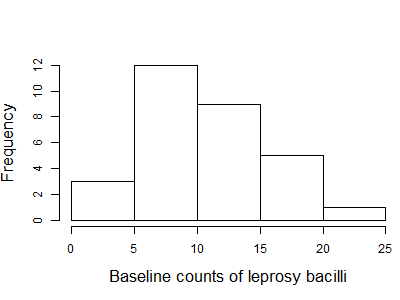
\includegraphics[width=.4\textwidth]{day_2_graphs_hist_example.png}}
\hspace{1cm}
\subfloat[Boxplot]{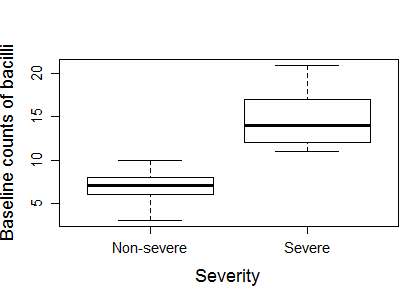
\includegraphics[width=.4\textwidth]{day_2_graphs_bplot_example.png}}

\subfloat[Scatterplot]{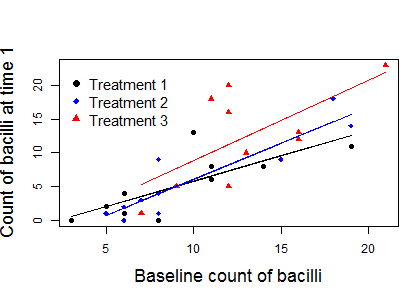
\includegraphics[width=.4\textwidth]{day_2_graphs_scatplot_example.png}}
\end{figure}
\end{frame}

\myframe{What do graphs tell us?}
\begin{itemize}
\item Histograms: summaries of one-dimensional distributions
\begin{itemize}
\item Counts or frequencies of each occurrence
\end{itemize}
\item[]
\item Boxplots: summaries of two-dimensional distributions
\begin{itemize}
\item measures of center (typically median)
\item[]
\item measures of spread (typically inter-quartile range)
\end{itemize}
\item[]
\item Scatterplots: summaries of two-dimensional distributions
\begin{itemize}
\item Can visualize the whole data
\item[]
\item Trends in two or more dimensions by using different colors/shapes for strata
\end{itemize}
\end{itemize}
\end{frame}

\section{Linear trends}
\myframe{Linear trends}
\begin{itemize}
\item A common way to describe data (think linear regression!)
\item[]
\item Lines are easy to compute
\begin{itemize}
\item Only need a point and a slope
\item[]
\item Two common forms of linear equations
\end{itemize}
\end{itemize}
\end{frame}

\myframe{Slope-intercept form}
\begin{itemize}
\item $y = mx + b$
\item[]
\item Slope: $m$
\begin{itemize}
\item Rate of change, i.e. how does $y$ change with each one unit change in $x$?
\item[]
\item Example: speed, the distance traveled with each unit change in time
\end{itemize}
\item[]
\item Intercept: $b$
\begin{itemize}
\item The point where the line crosses the $y-$axis
\end{itemize}
\end{itemize}
\end{frame}

\myframe{Slope-intercept form: determining a line}

\end{frame}

\myframe{Point-slope form}

\end{frame}

\myframe{Exercise: slopes and intercepts}

\end{frame}

\myframe{Solution: slopes and intercepts}

\end{frame}

\myframe{Creating a graph using an equation}

\end{frame}

\myframe{Reading an equation from a graph}

\end{frame}

\section{Quadratics}
\myframe{Quadratics}

\end{frame}

\myframe{Exercise: quadratics}

\end{frame}

\myframe{Solution: quadratics}

\end{frame}

\section{Shifting graphs}
\myframe{Shifting graphs}

\end{frame}

\myframe{Exercise: shifting graphs}

\end{frame}

\myframe{Solution: shifting graphs}

\end{frame}









\end{document}
